\documentclass[12pt]{article}
\usepackage{fancyhdr}
\usepackage{amsmath,amsfonts,enumerate}
\usepackage{color,graphicx}
\usepackage{tikz}
\usepackage{pgfplots}
\usepackage{listings}
\usepackage{algorithm}
\usepackage{algorithmic}
\usetikzlibrary{arrows,positioning,shapes,calc,matrix}
\pagestyle{fancy}
%%%%%%%%%%%%%%%%%%%%%%%%%%%%%%%%%%%%%%%%%%%%%%%%%
% Course customization based on Professor's teaching
%%%%%%%%%%%%%%%%%%%%%%%%%%%%%%%%%%%%%%%%%%%%%%%%%
\newcommand{\masunitnumber}{CENG 403}
\newcommand{\examdate}{January 2025}
\newcommand{\academicyear}{2024-2025}
\newcommand{\semester}{I}
\newcommand{\coursename}{Deep Learning - RNNs, Language Modeling \& Word Embeddings}
\newcommand{\numberofhours}{3}
%%%%%%%%%%%%%%%%%%%%%%%%%%%%%%%%%%%%%%%%%%%%%%%%%
% CUSTOM SPACING COMMANDS FOR ANSWER SPACES
%%%%%%%%%%%%%%%%%%%%%%%%%%%%%%%%%%%%%%%%%%%%%%%%%
\newcommand{\answerspace}[1]{\vspace{#1}}
\newcommand{\questionspace}{\vspace{3cm}}        
\newcommand{\subquestionspace}{\vspace{2.5cm}}   
\newcommand{\shortanswer}{\vspace{2cm}}          
\newcommand{\mediumanswer}{\vspace{3cm}}         
\newcommand{\longanswer}{\vspace{4cm}}           
\newcommand{\journalspace}{\vspace{4.5cm}}       
\newcommand{\codespace}{\vspace{5cm}}            
%%%%%%%%%%%%%%%%%%%%%%%%%%%%%%%%%%%%%%%%%%%%%%%%%
% Header setup
%%%%%%%%%%%%%%%%%%%%%%%%%%%%%%%%%%%%%%%%%%%%%%%%%
\lhead{}
\rhead{}
\chead{{\bf MIDDLE EAST TECHNICAL UNIVERSITY}}
\lfoot{}
\rfoot{}
\cfoot{}
\begin{document}
\setlength{\headsep}{5truemm}
\setlength{\headheight}{14.5truemm}
\setlength{\voffset}{-0.45truein}
\renewcommand{\headrulewidth}{0.0pt}
\begin{center}
SEMESTER \semester\ EXAMINATION \academicyear
\end{center}
\begin{center}
{\bf \masunitnumber\ -- \coursename}
\end{center}
\vspace{20truemm}
\noindent \examdate\hspace{45truemm} TIME ALLOWED: \numberofhours\ HOURS
\vspace{19truemm}
\hrule
\vspace{19truemm}
\noindent\underline{INSTRUCTIONS TO CANDIDATES}
\vspace{8truemm}
%%%%%%%%%%%%%%%%%%%%%%%%%%%%%%%%%%%%%%%%%%%%%%%%%%%%%%
% Instructions based on professor's emphasis
%%%%%%%%%%%%%%%%%%%%%%%%%%%%%%%%%%%%%%%%%%%%%%%%%%%%%%
\begin{enumerate}
\item This examination paper contains {\bf SIX (6)} questions and comprises 
{\bf EIGHT (8)} printed pages.
\item Answer all questions. 
The marks for each question are indicated at the beginning of each question.
\item Answer each question beginning on a {\bf FRESH} page of the answer book.
\item This {\bf IS NOT an OPEN BOOK} exam.
\item Show clear reasoning for your answers, especially intuitive explanations.
\item For algorithms, provide step-by-step explanations as taught in lectures.
\item Draw diagrams where requested and explain information flow clearly.
\item Connect concepts to modern applications (LLMs, etc.) where relevant.
\end{enumerate}
%%%%%%%%%%%%%%%%%%%%%%%%%%%%%%%%%%%%%%%%%%%%%%%%%
% New page for questions
%%%%%%%%%%%%%%%%%%%%%%%%%%%%%%%%%%%%%%%%%%%%%%%%%
\newpage
\lhead{}
\rhead{\masunitnumber}
\chead{}
\lfoot{}
\cfoot{\thepage}
\rfoot{}
\setlength{\footskip}{45pt}
%%%%%%%%%%%%%%%%%%%%%%%%%%%%%%%%%%%%%%%%%%%%%%%%%%
% EXAM QUESTIONS BASED ON PROFESSOR'S TEACHING
%%%%%%%%%%%%%%%%%%%%%%%%%%%%%%%%%%%%%%%%%%%%%%%%%%

\paragraph{Question 1. RNN Backpropagation and Weight Sharing}\hfill (25 marks)\\
Based on the professor's explanation of how RNNs work as "feedforward networks with weight sharing across time."

\begin{enumerate}[(a)]
    \item The professor emphasized that "we need to be careful about weight sharing when calculating gradients." Explain why we must sum gradients from all time steps for a single weight parameter in an RNN. Use a concrete example with 3 time steps. \hfill (8 marks)
    
    \mediumanswer
    
    \item During backpropagation through time, the professor stressed that "we need to start from the end because earlier copies contribute to all following time steps." Draw and explain the gradient flow through an unfolded RNN showing why this order is essential. \hfill (10 marks)
    
    \begin{center}
    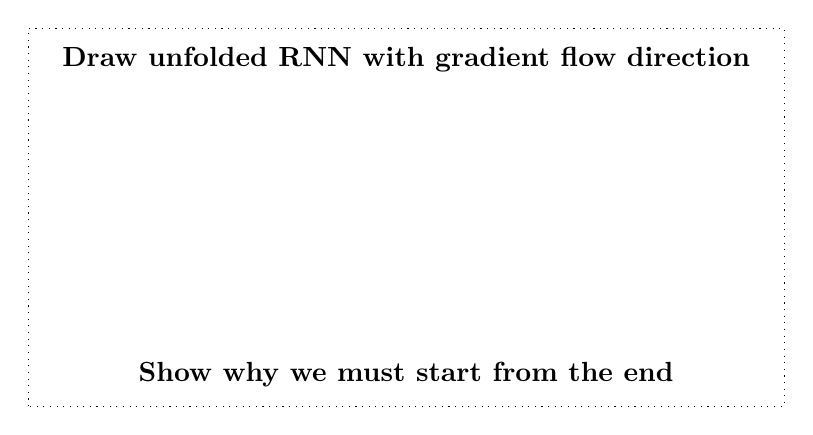
\begin{tikzpicture}[scale=0.8]
        % Students should draw unfolded RNN with gradient flow
        \draw[dotted] (0,0) rectangle (12,6);
        \node at (6,5.5) {\textbf{Draw unfolded RNN with gradient flow direction}};
        \node at (6,0.5) {\textbf{Show why we must start from the end}};
    \end{tikzpicture}
    \end{center}
    
    \shortanswer
    
    \item The professor mentioned that RNNs suffer from "exploding gradient problem if weight norms are large, vanishing gradient problem if norms are small." Explain the mathematical reasoning behind both problems and why LSTM addresses these issues. \hfill (7 marks)
    
    \mediumanswer
\end{enumerate}

\newpage
\paragraph{Question 2. Autoregressive Language Modeling}\hfill (20 marks)\\
The professor stated: "This is how large language models are trained as well - just to predict the next character."

\begin{enumerate}[(a)]
    \item Define autoregressive modeling as explained by the professor. Write the mathematical formulation for modeling $P(x_t | x_{t-1}, x_{t-2}, \ldots, x_1)$ and explain why this is considered "self-supervised learning." \hfill (8 marks)
    
    \mediumanswer
    
    \item The professor explained the difference between training and inference in language models. Complete the diagram below showing both processes for the sequence "hello": \hfill (12 marks)
    
    \begin{center}
    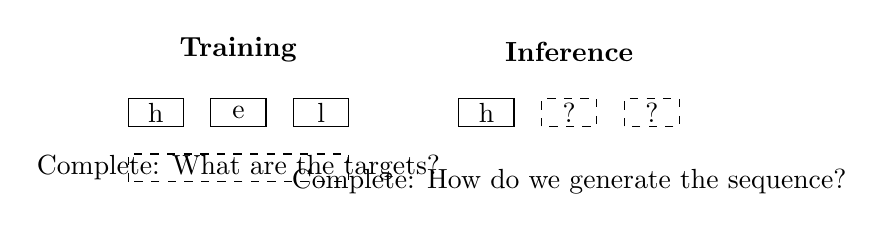
\begin{tikzpicture}[scale=0.7]
        % Training process
        \node[above] at (2,3) {\textbf{Training}};
        \draw (0,2) rectangle (1,2.5);
        \node at (0.5,2.25) {h};
        \draw (1.5,2) rectangle (2.5,2.5);
        \node at (2,2.25) {e};
        \draw (3,2) rectangle (4,2.5);
        \node at (3.5,2.25) {l};
        
        % Students complete this
        \draw[dashed] (0,1) rectangle (4,1.5);
        \node at (2,1.25) {Complete: What are the targets?};
        
        % Inference process  
        \node[above] at (8,3) {\textbf{Inference}};
        \draw (6,2) rectangle (7,2.5);
        \node at (6.5,2.25) {h};
        \draw[dashed] (7.5,2) rectangle (8.5,2.5);
        \node at (8,2.25) {?};
        \draw[dashed] (9,2) rectangle (10,2.5);
        \node at (9.5,2.25) {?};
        
        \node at (8,1) {Complete: How do we generate the sequence?};
    \end{tikzpicture}
    \end{center}
    
    \shortanswer
\end{enumerate}

\newpage
\paragraph{Question 3. Character-Level Implementation Details}\hfill (22 marks)\\
Based on the professor's detailed walkthrough of the "hello" example with 4-character vocabulary.

\begin{enumerate}[(a)]
    \item The professor showed how to use one-hot encodings for characters h, e, l, o. Given the string "hello", create the complete training data with inputs and targets, including start and end tokens as explained in class. \hfill (8 marks)
    
    \journalspace
    
    \item Follow the professor's example: given input character 'h' with one-hot encoding [1,0,0,0], weight matrix $W_1$ (3×4), and hyperbolic tangent activation, show the complete forward pass to predict the next character. Explain each step as the professor did. \hfill (10 marks)
    
    \mediumanswer
    
    \item The professor emphasized that during inference "we use the predicted value as input for the next time step, even if it's incorrect." Explain why this creates a potential problem and how it relates to error propagation in sequence generation. \hfill (4 marks)
    
    \shortanswer
\end{enumerate}

\newpage
\paragraph{Question 4. Beam Search Algorithm}\hfill (25 marks)\\
The professor explained beam search as an alternative to "greedy approach where we just take the character with highest probability."

\begin{enumerate}[(a)]
    \item Implement the beam search algorithm as taught by the professor. Given the probability distributions below for 3 time steps with vocabulary [A, B, C], show the complete beam search process with beam size k=2: \hfill (15 marks)
    
    \begin{center}
    \begin{tabular}{|c|c|c|c|}
    \hline
    Time Step & P(A) & P(B) & P(C) \\
    \hline
    t=1 & 0.6 & 0.3 & 0.1 \\
    t=2 (after A) & 0.2 & 0.5 & 0.3 \\
    t=2 (after B) & 0.4 & 0.1 & 0.5 \\
    t=3 (after AA) & 0.1 & 0.2 & 0.7 \\
    t=3 (after AB) & 0.3 & 0.3 & 0.4 \\
    \hline
    \end{tabular}
    \end{center}
    
    Show the tree expansion and final top-2 sequences with their combined scores.
    
    \codespace
    
    \item The professor mentioned that "beam search during training is very expensive because you need to unfold this tree." Explain why beam search is typically used only during inference and what computational challenges it would create during training. \hfill (10 marks)
    
    \mediumanswer
\end{enumerate}

\newpage
\paragraph{Question 5. Word-Level Challenges and Embeddings}\hfill (28 marks)\\
The professor explained the transition from character-level to word-level modeling and the need for word embeddings.

\begin{enumerate}[(a)]
    \item The professor stated that English has "170,000 different words" making one-hot encoding impractical. Calculate the number of parameters needed for: \hfill (8 marks)
    \begin{itemize}
        \item Input layer: 170,000-dimensional one-hot to 512-dimensional hidden layer
        \item Compare this with character-level (30 characters to 512 dimensions)
        \item Explain why this creates a "huge" parameter problem as the professor mentioned
    \end{itemize}
    
    \mediumanswer
    
    \item The professor emphasized that "in one-hot representation every word is equally distant to each other." Explain why this is problematic for semantic understanding and how word embeddings solve this issue. Use the examples the professor gave: "running and jogging should be close vs. running and swimming." \hfill (10 marks)
    
    \mediumanswer
    
    \item Design the CBOW (Continuous Bag of Words) architecture as explained by the professor. For the sentence "I like running every day" with target word "running", show: \hfill (10 marks)
    \begin{itemize}
        \item Context words and their representation
        \item How the weight matrix W1 stores embeddings
        \item Why "the network is forced to learn word vectors that capture relevance"
    \end{itemize}
    
    \mediumanswer
\end{enumerate}

\newpage
\paragraph{Question 6. Deep Understanding and Modern Connections}\hfill (30 marks)\\
Based on the professor's connections between classical methods and modern applications.

\begin{enumerate}[(a)]
    \item The professor made a key connection: "The prompts that you provide to LLMs are actually the starting sequences that you provide to an RNN-like architecture." Explain this connection and how modern LLMs relate to the autoregressive character prediction discussed in class. \hfill (10 marks)
    
    \mediumanswer
    
    \item Analyze the professor's examples of character-level RNN outputs (Shakespeare, Wikipedia, LaTeX). Explain what these results demonstrate about: \hfill (12 marks)
    \begin{itemize}
        \item Learning syntax without explicit supervision
        \item Generalization vs. memorization (the professor's "overfitting" discussion)
        \item Why the professor called these results "striking" for such simple models
    \end{itemize}
    
    \longanswer
    
    \item The professor showed word embedding arithmetic: "Paris - France + Italy = Rome." Explain: \hfill (8 marks)
    \begin{itemize}
        \item Why this works mathematically in embedding space
        \item How the CBOW training creates these relationships
        \item Give two more examples of word arithmetic that should work
    \end{itemize}
    
    \mediumanswer
\end{enumerate}

\vfill
\begin{center}{\bf END OF PAPER}\end{center}
\end{document}